%************************************************
\chapter{Learning to Accomplish Goals}\label{ch:learning_to_accomplish_goals}
%************************************************

\begin{quote}
  Problem-solvers must find relevant data.  How does the human mind
  retrieve what it needs from among so many millions of knowledge items?
  Different AI systems have attempted to use a variety of different
  methods for this.  Some assign keywords, attributes, or descriptors to
  each item and then locate data by feature-matching or by using more
  sophisticated associative data-base methods.  Others use
  graph-matching or analogical case-based adaptation.  Yet others try to
  find relevant information by threading their ways through systematic,
  usually hierarchical classifications of knowledge---sometimes called
  ``ontologies''.  But, to me, all such ideas seem deficient because it
  is not enough to classify items of information simply in terms of the
  features or structures of those items themselves.  This is because we
  rarely use a representation in an intentional vacuum, but we always
  have goals---and two objects may seem similar for one purpose but
  different for another purpose.
\end{quote}
\begin{flushright}
  --- \defcitealias{minsky:1991}{Marvin Minsky}\citetalias{minsky:1991}
\end{flushright}

In this introductory chapter I will give an overview of the problem of
reflectively learning to accomplish goals.  First, I will develop the
assumption that any process that I choose in my system can be
reflectively monitored and useful information, e.g. beginning and
ending times, will be temporarily stored.  In other words, I assume
that my system natively supports procedural reflection for all
processes.  Given this assumption, I show in this chapter that the
problem of building a system that learns to accomplish goals in its
environment becomes a simple loop-less causal structure involving at
least four different types of learning that together, through time,
complete a circle of causal learning from goals through actions to
physical states and back to goals, but because of time, causality is
still in an ordered lattice structure beginning with goals as the
causal roots for all other knowledge.

In later chapters I will introduce experiments I have performed in
different physical problem simulations.  The first is a simple
proof-of-concept demonstration of my reflective learning algorithm in
a blocks world problem domain.  Also, I show my reflective
architecture extended to a larger physical reasoning domain, including
multiple agents learning to cook together in a kitchen environment.
In this larger problem space, agents can communicate high-level
procedures specified in a simple programming language that is shared
by the agents, and refers to both mental and physical actions of the
agents.

\section{The Agent-Environment Model}

\begin{figure}[bth]
  \center
  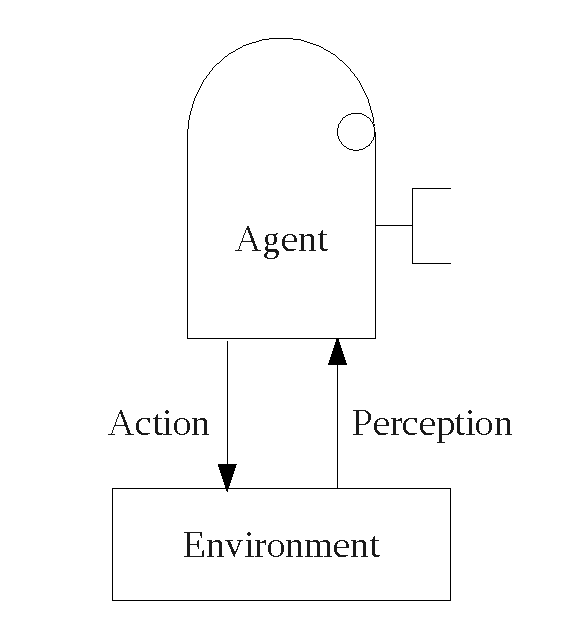
\includegraphics[height=5cm]{gfx/agent_environment}
  \caption[The agent-environment model]{The agent-environment model.}
  \label{fig:agent_environment}
\end{figure}

Figure~\ref{fig:agent_environment} shows the basic agent-environment
model.  In this model, I make a distinction between the environment
and the agent.  At any given time, the agent and the environment are
each represented as a specific static form of data.  Further, these
representations change over time, according to a given transfer
function.  I will treat this system as a deterministic system,
although one could imagine adding random variables to the transfer
function: the basic theory is the same.  It is easier to add
randomness to a deterministic theory than the opposite.  There are
also many benefits to developing a deterministic model with perhaps a
pseudorandom aspect because this allows for the repeatability of
scientific experiments, for which the model may be used as a metric.
The two processes communicate information along two channels: (1) an
action channel from the agent to the environment, and (2) a perception
channel from the environment to the agent.


\section{The State-Action Model}
\label{sec:state_action_model}

\begin{figure}[bth]
  \center
  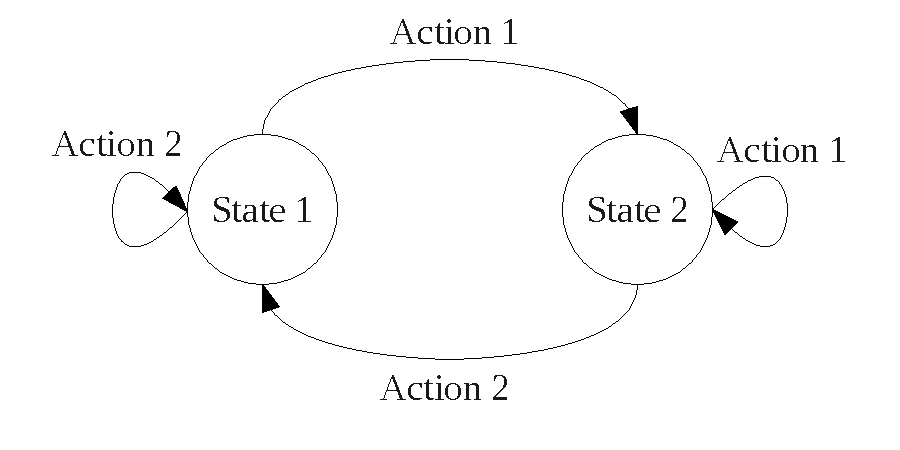
\includegraphics[width=6cm]{gfx/state_action}
  \caption[The state-action model]{The state action model.  Two states
    are represented by nodes and two actions are represented by edges
    from each of the two states.}
  \label{fig:state_action}
\end{figure}

The agent is in an environment, which is in a specific state.  My
agent performs an action, which can affect the state of the
environment.  Figure~\ref{fig:state_action} shows a simple \ac{FSM}
state-action model, which has two states for the environment and two
actions for the agent to perform in each of these states.  The
state-action model is a simple model for how actions map to changes in
the state of the environment.


\section{A Multiple Agent-Environment Model}

\begin{figure}[bth]
  \center
  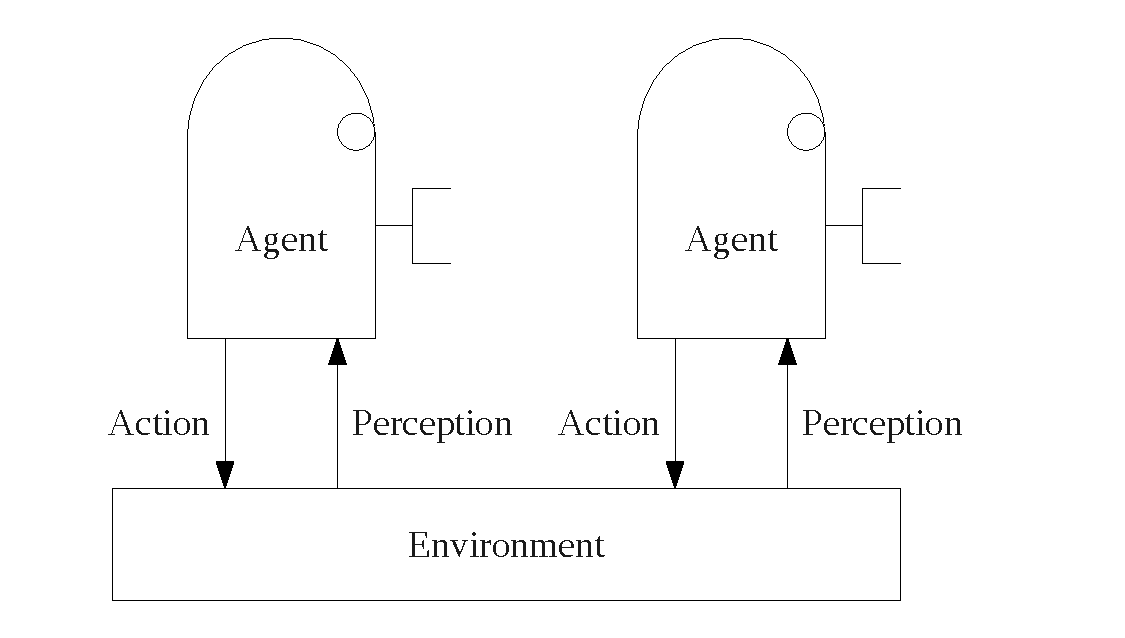
\includegraphics[height=5cm]{gfx/multiple_agent_environment}
  \caption[The multiple agent environment model]{The multiple agent environment model.}
  \label{fig:multiple_agent_environment}
\end{figure}

In order to model social intelligence, we introduce the multiple agent
environment model shown in
Figure~\ref{fig:multiple_agent_environment}.


\section{Agent Process Communication}

Because agent processes can only directly act on and perceive the
environment, all communication between agent processes must occur
through the environment process.  We assume that agents can
communicate some form of symbolic knowledge structure in the absence
of noise.  These representations are used to communicate processes
from one agent to another.  Specific examples of such a process
representation that we have used in our experiments are described in
more detail in
Sections~\ref{sec:serial_process_representation}--\ref{sec:parallel_process_representation}.


\section{A Relational State Representation}

\begin{figure}[bth]
  \center
  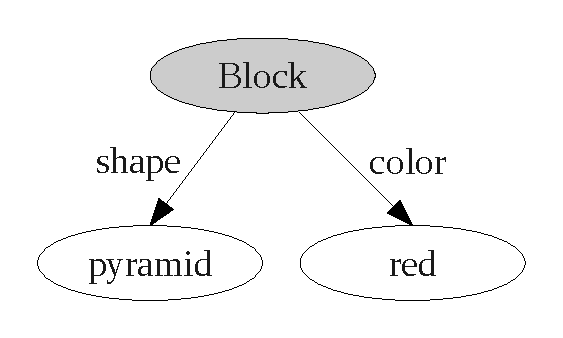
\includegraphics[height=3cm]{gfx/frame_representation}
  \caption[Frame-based relational representation.]{Frame-based relational representation.}
  \label{fig:frame_representation}
\end{figure}

See Figure~\ref{fig:frame_representation}.

\section{Introducing Reflection Early in the Process}

Now, I have introduced my problem as being divided into at least two
processes, at least one agent process and an environment process.
Further, I have introduced how a basic process may be thought of as an
\ac{FSM}.  At this point, I introduce a model for keeping track of the
changes in a computational process: reflective knowledge.  I
purposefully make this assumption before I define the details of the
agent model process because, in my approach, I would like to
reflectively reason about potentially any aspect of this agent
process.

\section{Reflective Knowledge}

\begin{figure}[bth]
  \center
  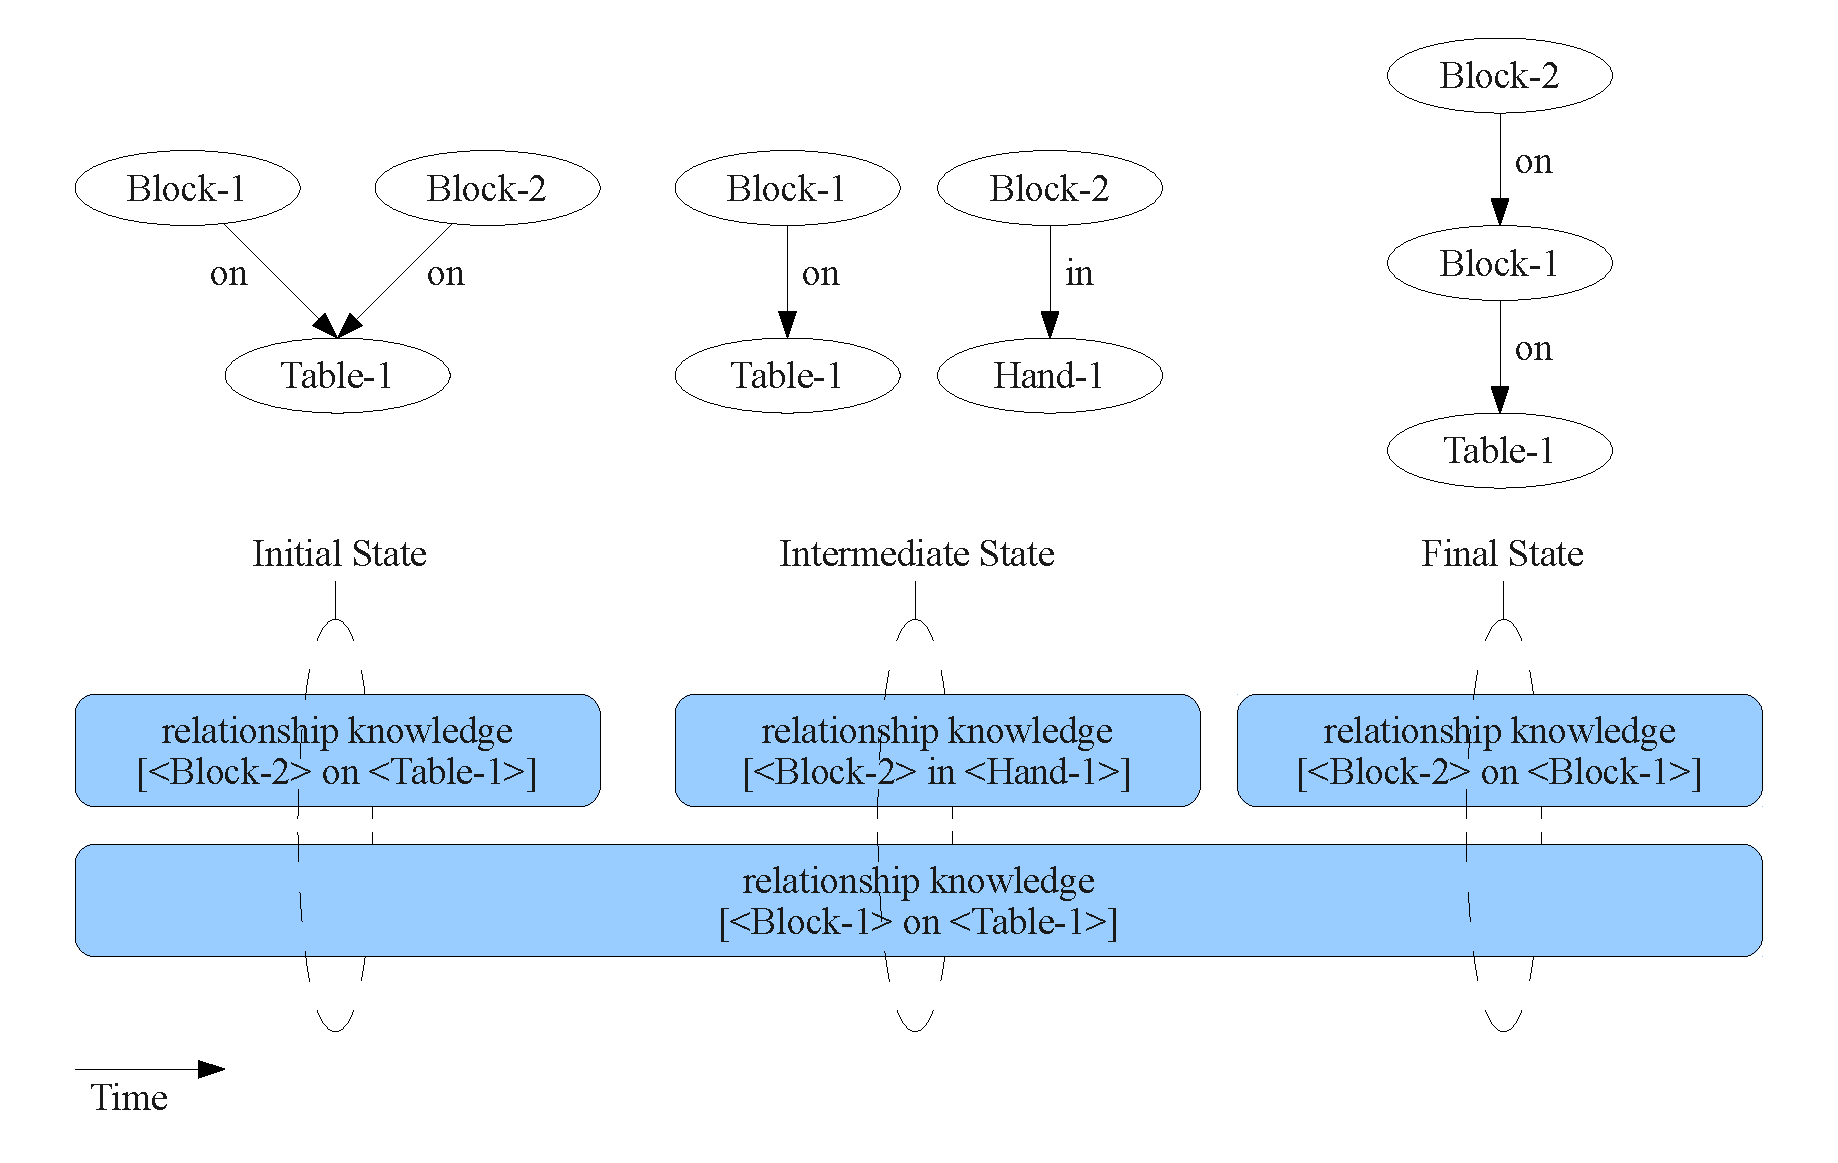
\includegraphics[width=12cm]{gfx/reflective_event_representation}
  \caption[A reflective event representation]{A reflective event representation shows the changes in a labeled graph.}
  \label{fig:reflective_event_representation}
\end{figure}


While the term meta-knowledge is used to describe the very general
idea of knowledge about knowledge, I use the term reflective
knowledge to refer to the specific type of meta-knowledge that refers
to knowledge about the changes to a knowledge structure.  If I keep
track of the changes to a knowledge structure, I can later integrate
these changes in order to obtain an equivalent form of that knowledge
structure as it was at any point in the past.

While this relatively simple definition of how to reflective over a
computational process fulfills my purpose of an introductory
explanation, see Section~\ref{sec:what_is_a_computer} for a discussion
about approaching more realistic models of computation that include
more of the engineering details of efficiently controlling modern
computer hardware systems.


\section{Frame Perceptions}

\begin{figure}[bth]
  \center
  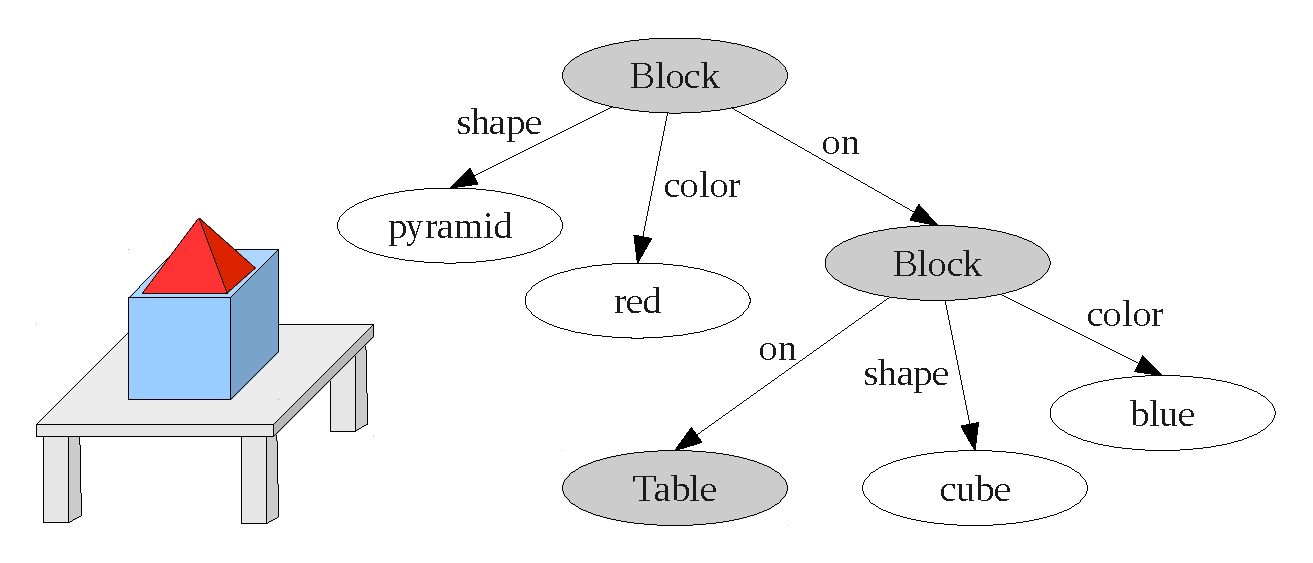
\includegraphics[height=5cm]{gfx/frame_perception}
  \caption[Collections of frames used as perceptual input to agent.]{Collections of frames used as perceptual input to agent.}
  \label{fig:frame_perception}
\end{figure}

See Figure~\ref{fig:frame_perception}.


\section{Partially Observable State Model}

\begin{figure}[bth]
  \center
  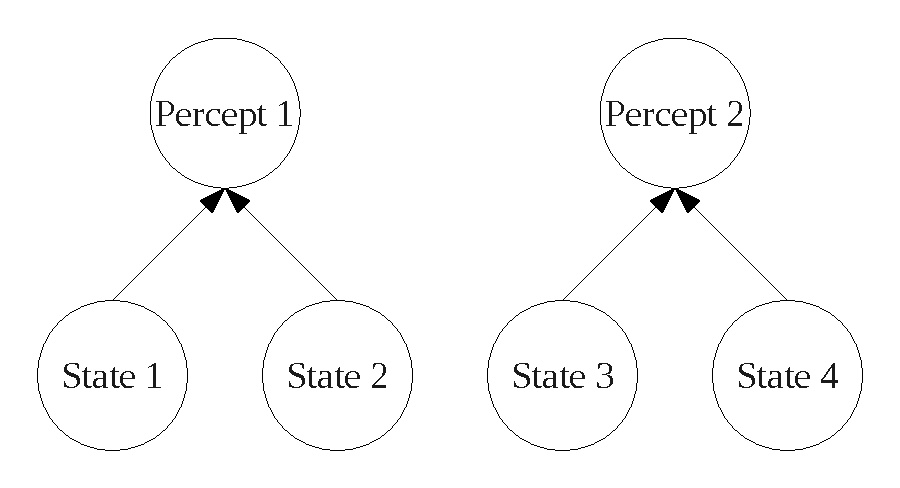
\includegraphics[width=6cm]{gfx/partially_observable}
  \caption[The partially observable state model]{The partially observable model.}
  \label{fig:partially_observable}
\end{figure}

The agent process does not have complete access to the state of its
environment.  The agent's perceptual stream of information depends on
the state of the environment, but it is a function of the environment
and not the actual state of the environment.  In other words, the
perceptual state that is communicated from the environment to the
agent is an injective function mapping the environment to the
perception of the agent.


\section{Partial Frame Perceptions}

\begin{figure}[bth]
  \center
  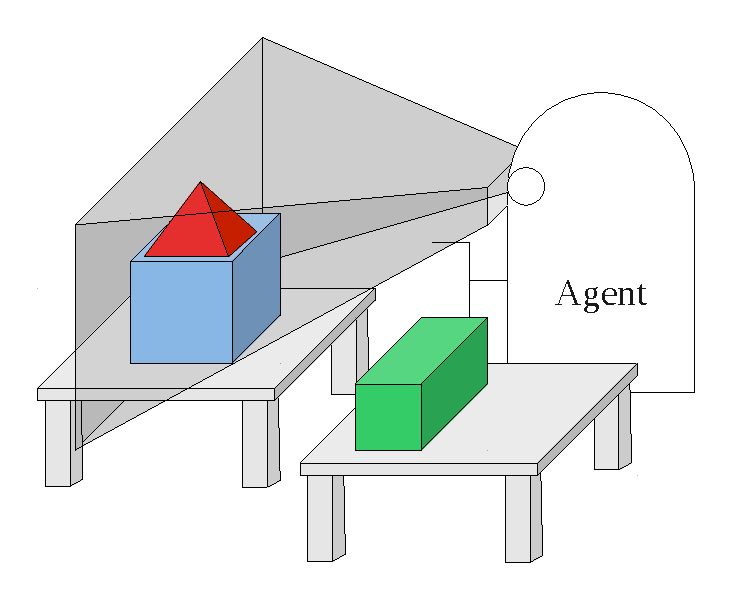
\includegraphics[height=5cm]{gfx/partial_frame_perception}
  \caption[The state of the environment is only partially
    observable.]{The state of the environment is only partially
    observable.}
  \label{fig:partial_frame_perception}
\end{figure}

See Figure~\ref{fig:partial_frame_perception}.


\section{Agent Abstract Physical Model}

\begin{figure}[bth]
  \center
  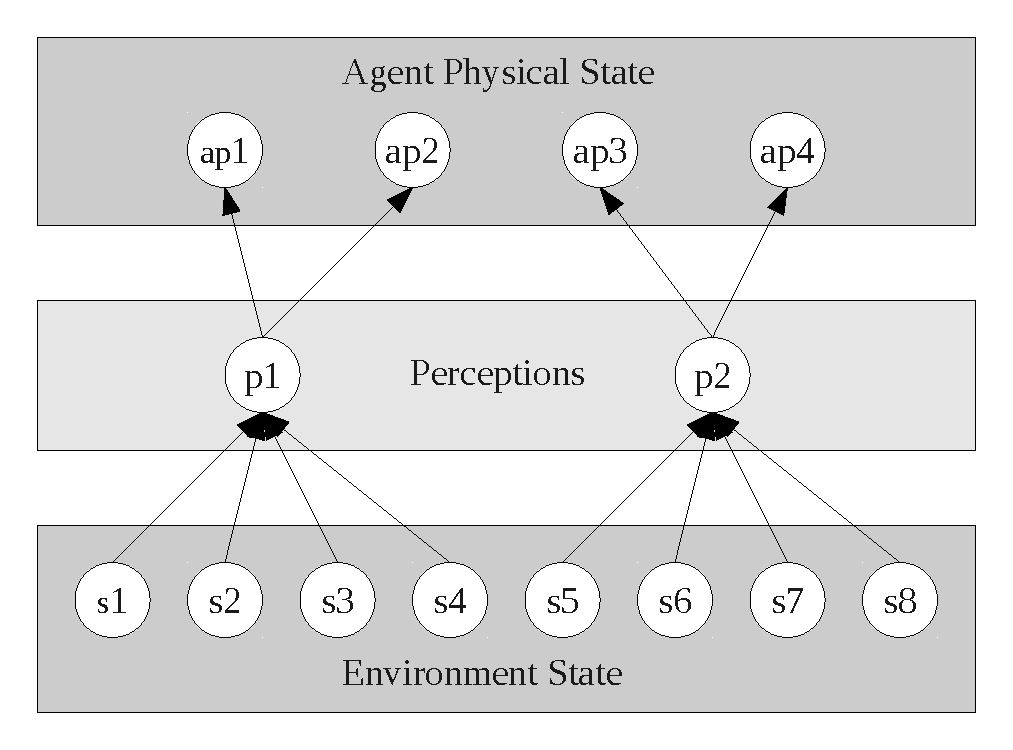
\includegraphics[width=8cm]{gfx/environment_perception_physical}
  \caption[The agent has an abstract physical model of the
    environment.]{The agent has an abstract physical model of the
    environment.}
  \label{fig:environment_perception_physical}
\end{figure}

See Figure~\ref{fig:environment_perception_physical}.


\section{A Physical Goal Representation}

\begin{figure}[bth]
  \center
  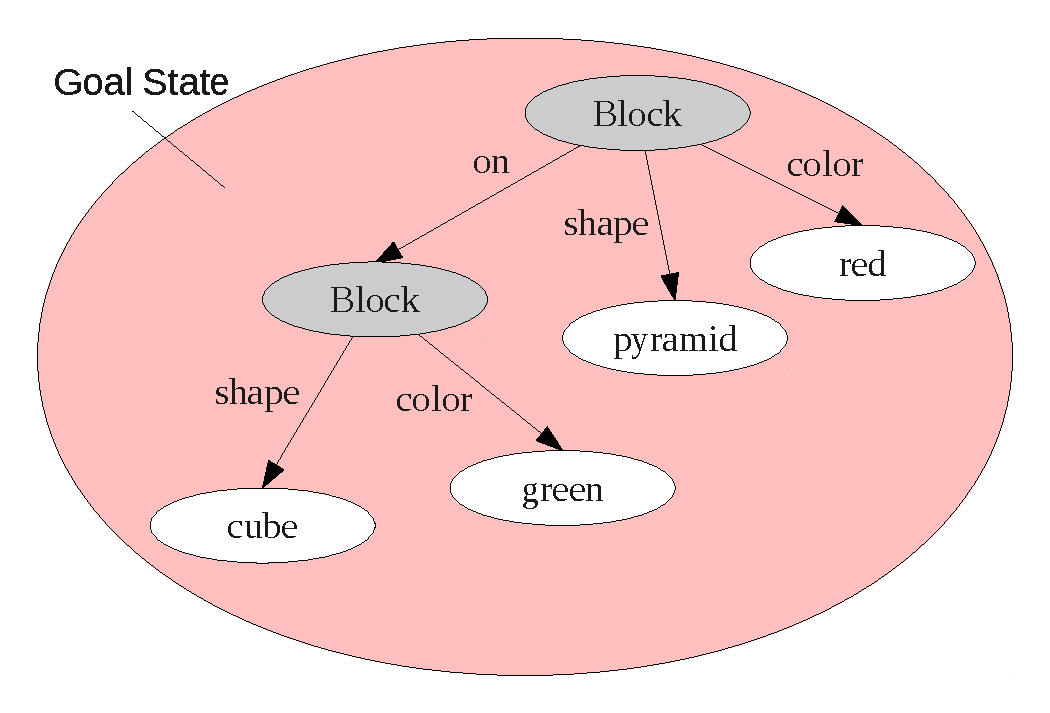
\includegraphics[height=4cm]{gfx/goal_state}
  \caption[A physical goal representation]{A physical goal
    representation is a structural relationship that may or may not
    currently exist within the physical knowledge base.}
  \label{fig:goal_state}
\end{figure}

See Figure~\ref{fig:goal_state}.


\section{Reflective Goal-Oriented Learning}

\begin{figure}[bth]
  \center
  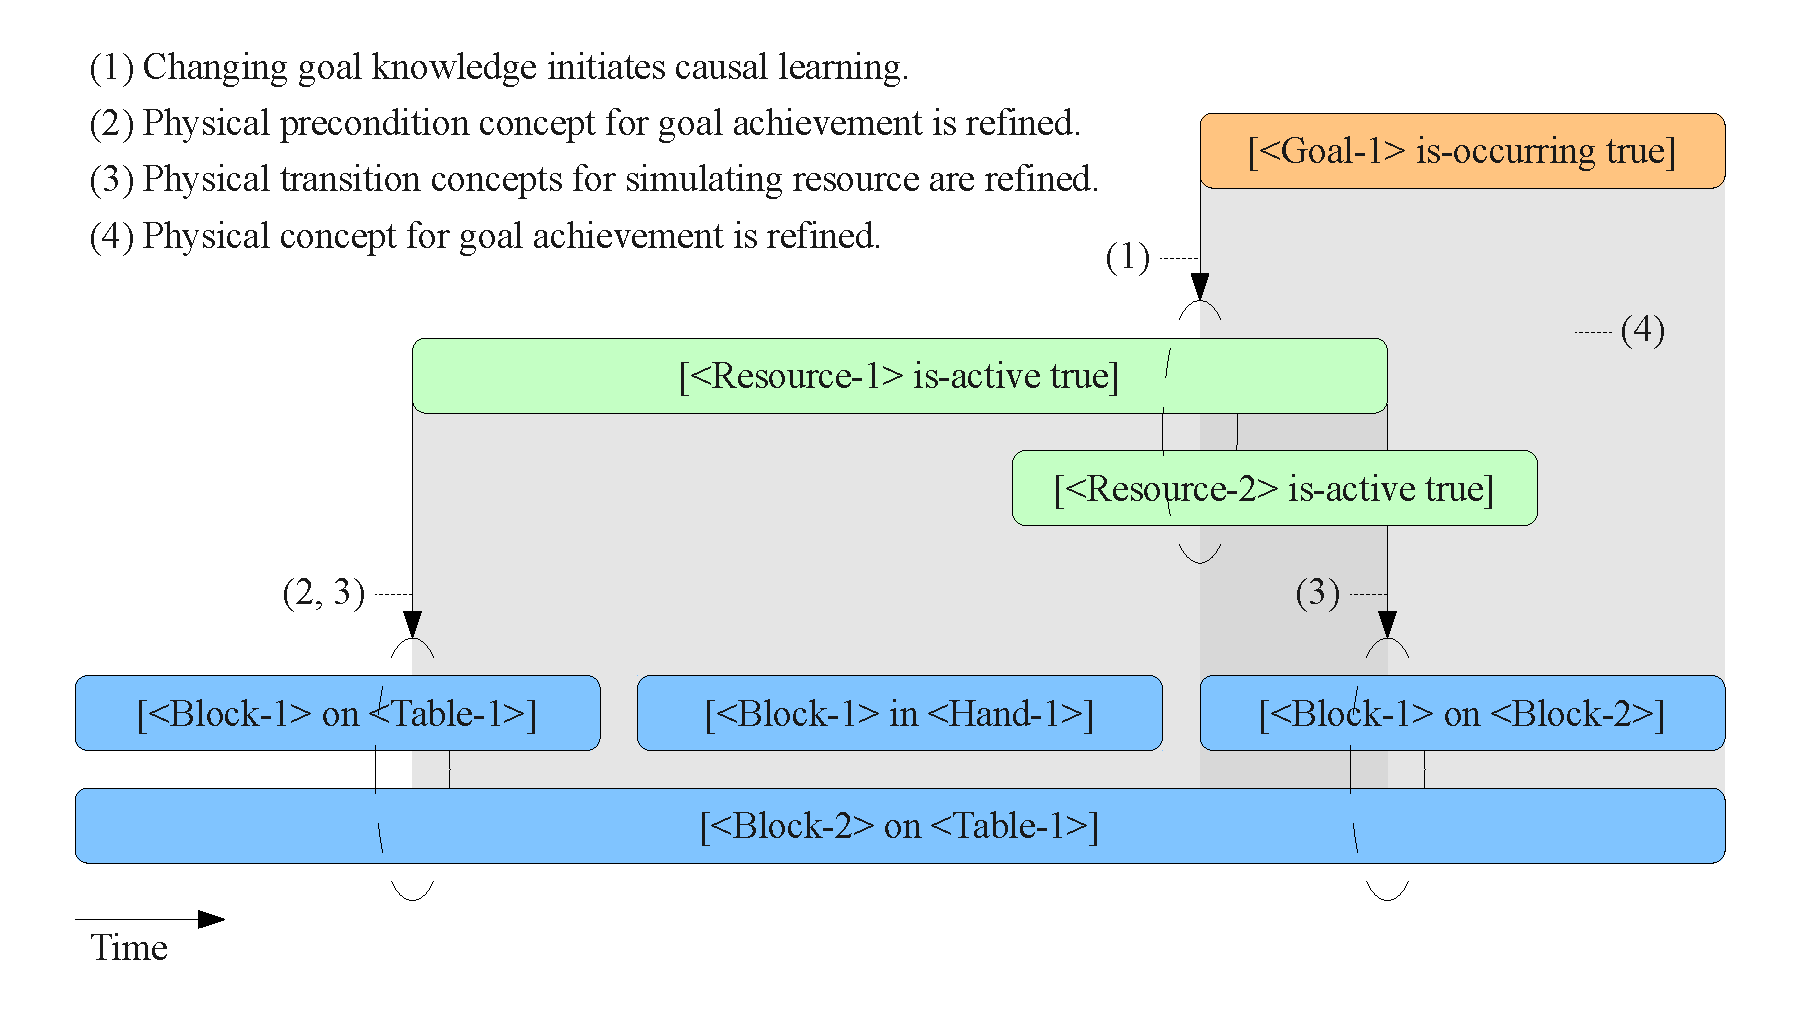
\includegraphics[width=12cm]{gfx/learning_to_plan}
  \caption[Learning to plan toward goals]{Learning to plan toward
    goals is naturally represented in a reflective event
    representation.}
  \label{fig:learning_to_plan}
\end{figure}

A system without a goal has no reason to learn the effects of its
actions.  Figure~\ref{fig:learning_to_plan} shows how the process of
learning causal models relating reflective states to physical states
is a fundamentally goal-driven process.

\marginpar{\emph{learning goal}: focusing learning on a subset of the state space.}


\section{Learning Trans-Frames for Events}
\label{sec:learning_trans_frames_for_events}

\begin{figure}[bth]
  \center
  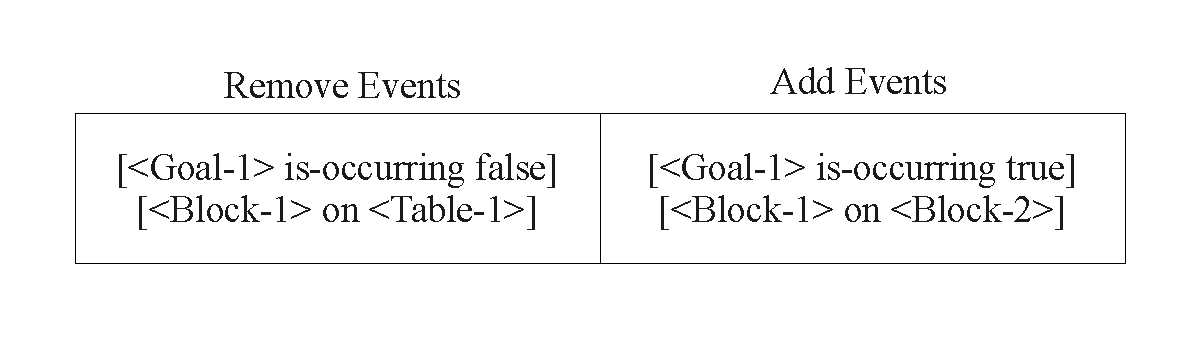
\includegraphics[width=10cm]{gfx/transframe}
  \caption[A trans-frame for an event]{A trans-frame for an event is a
    list of differences in knowledge between the beginning and ending
    of the event.}
  \label{fig:transframe}
\end{figure}

See Figure~\ref{fig:transframe}.  Also, trans-frames of trans-frames
can be thought of as a form of analogical transfer, which I further
discuss in
Section~\ref{sec:learning_analogies_as_differences_of_differences}.


\section{Partially-Ordered Plan Representation}

\begin{figure}[bth]
  \center
  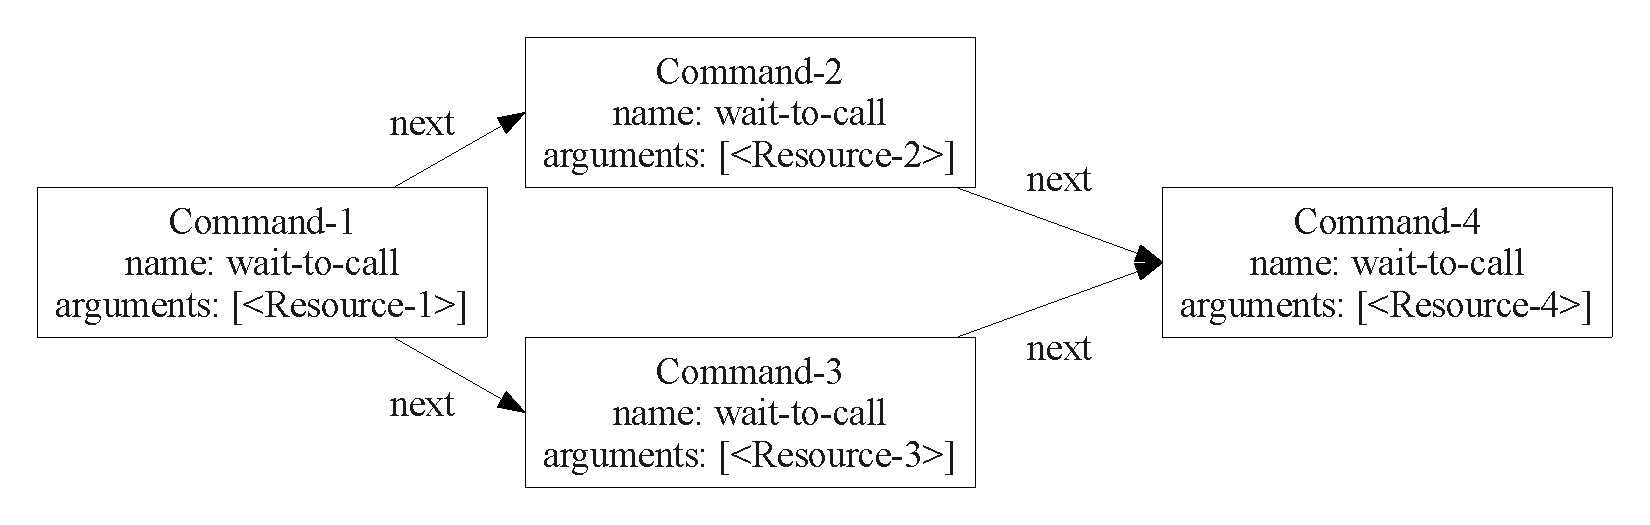
\includegraphics[width=11cm]{gfx/serial_and_parallel_plan}
  \caption[A partially-ordered plan with serial and parallel
    components.]{A partially-ordered plan representation containing
    serial and parallel components.}
  \label{fig:serial_and_parallel_plan}
\end{figure}

The partially-ordered plan representation allows a partially-ordered
temporal organization for a set of commands.  A plan with a
branch-and-join control structure is shown in
Figure~\ref{fig:serial_and_parallel_plan}.


\section{Inferring the Effects of a Plan}
\label{sec:inferring_the_effects_of_a_plan}

\begin{figure}[bth]
  \center
  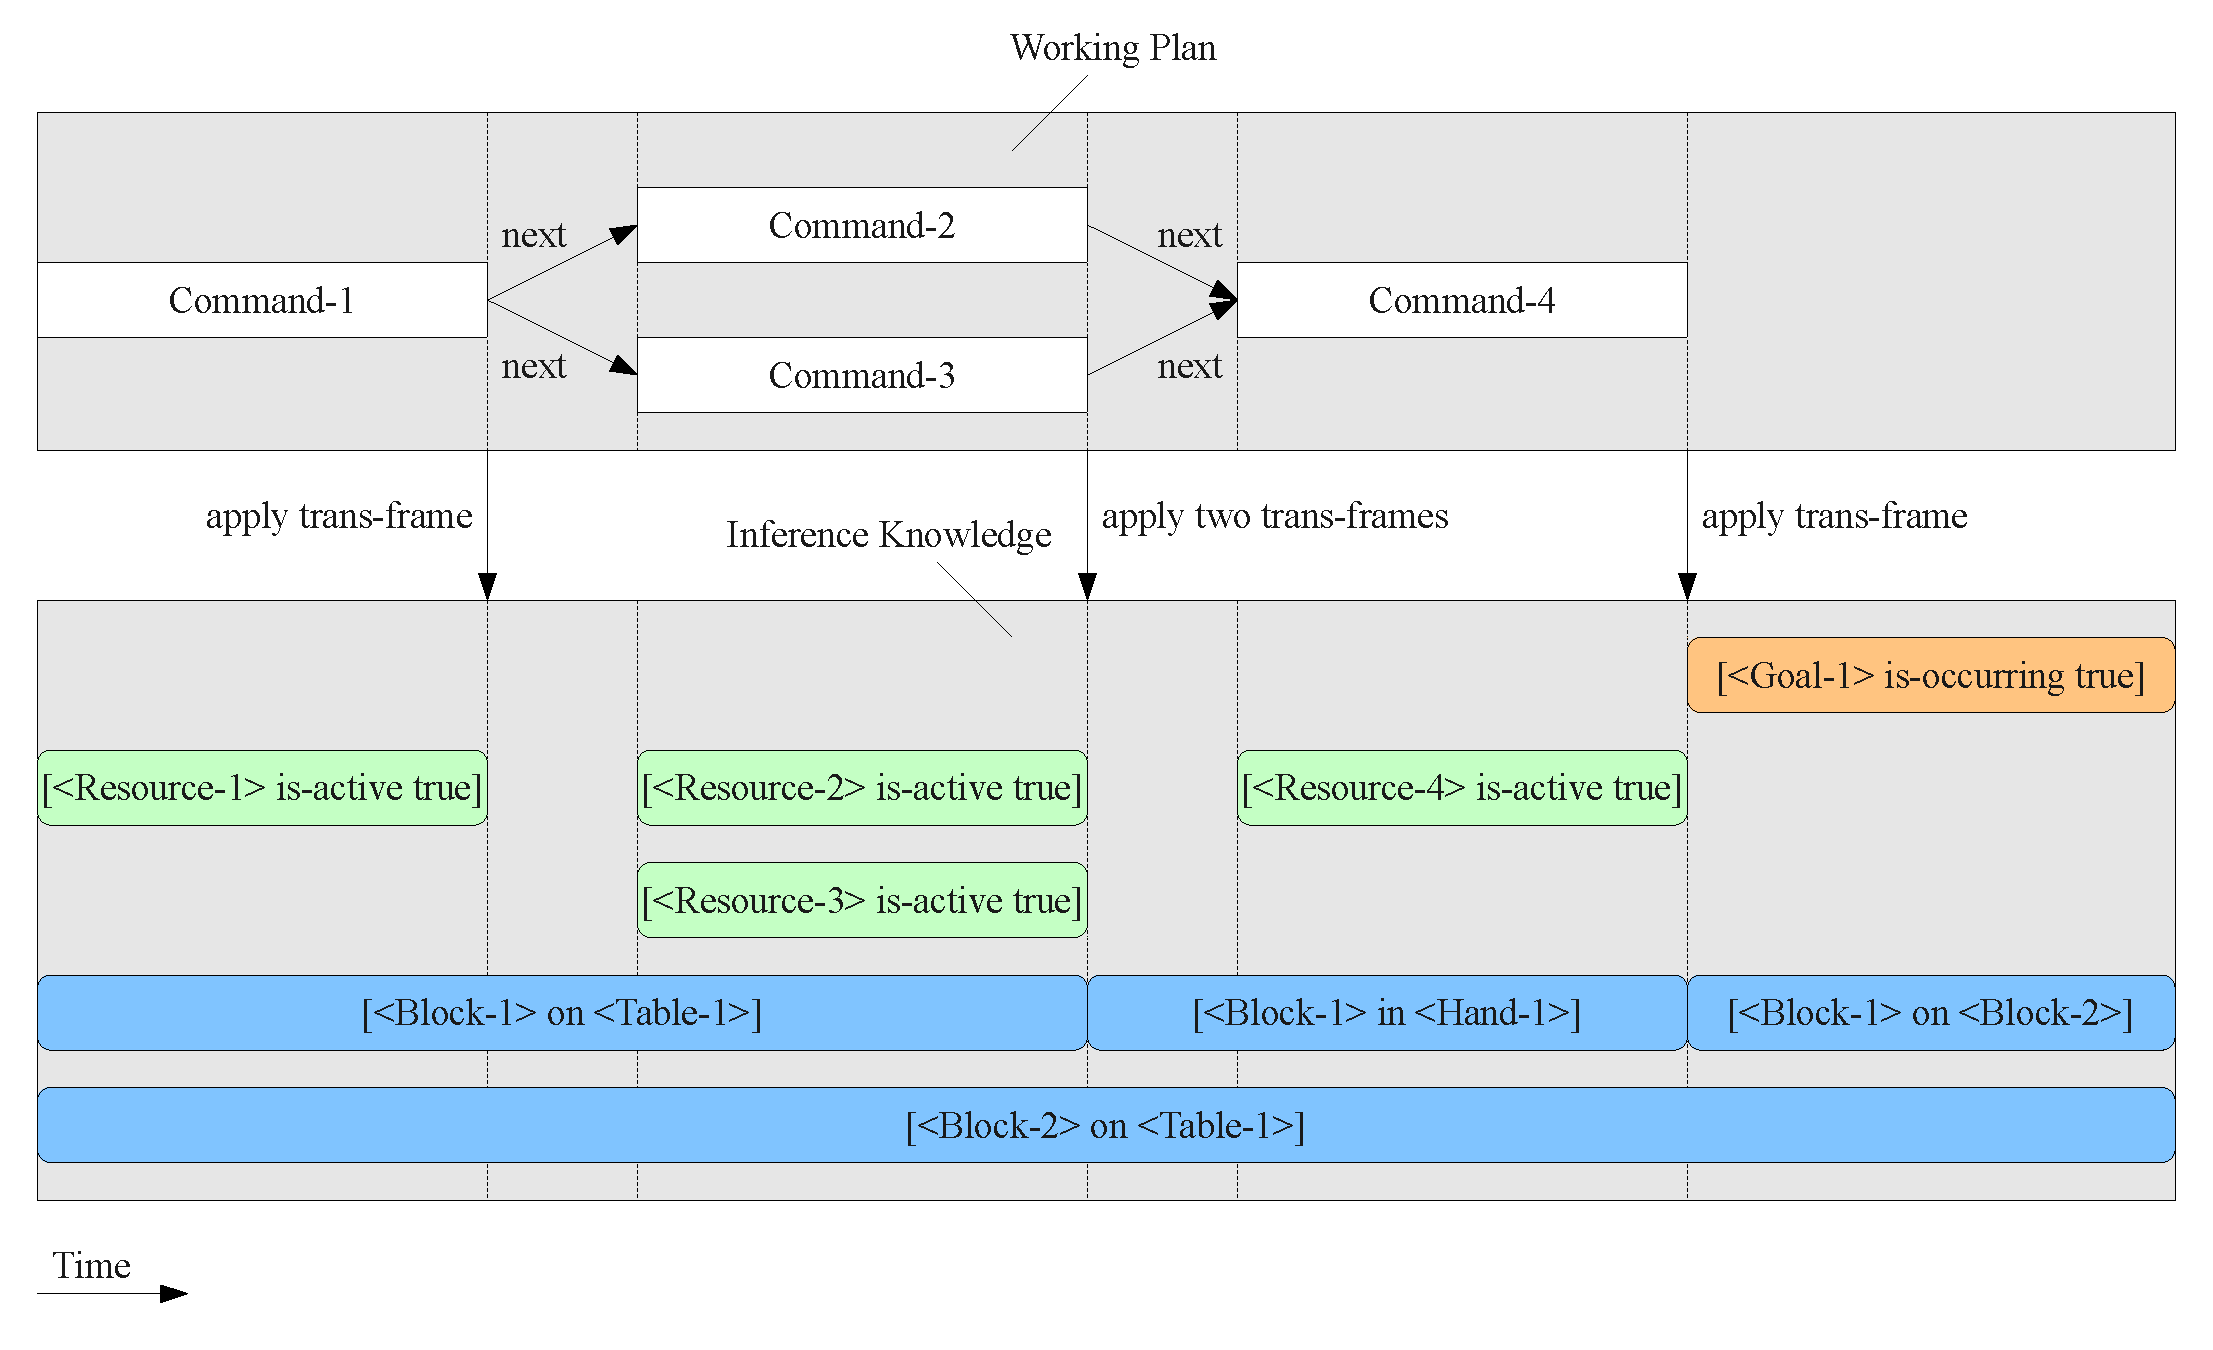
\includegraphics[width=11cm]{gfx/infer_plan_effects}
  \caption[Inferring the effects of a plan.]{Inferring the effects of
    a plan.}
  \label{fig:infer_plan_effects}
\end{figure}

The planning process requires an inference algorithm to infer future
and past states based on cause-effect relationships between reflective
knowledge and physical knowledge.  Figure~\ref{fig:infer_plan_effects}
shows a possible inference for a given plan.  There are many ways to
plan and the specific planning system that I have implemented for my
experiments is discussed further in
Section~\ref{sec:details_of_inferring_the_effects_of_a_plan}.


\section{Planning Machine Operations}

\begin{figure}[bth]
  \center
  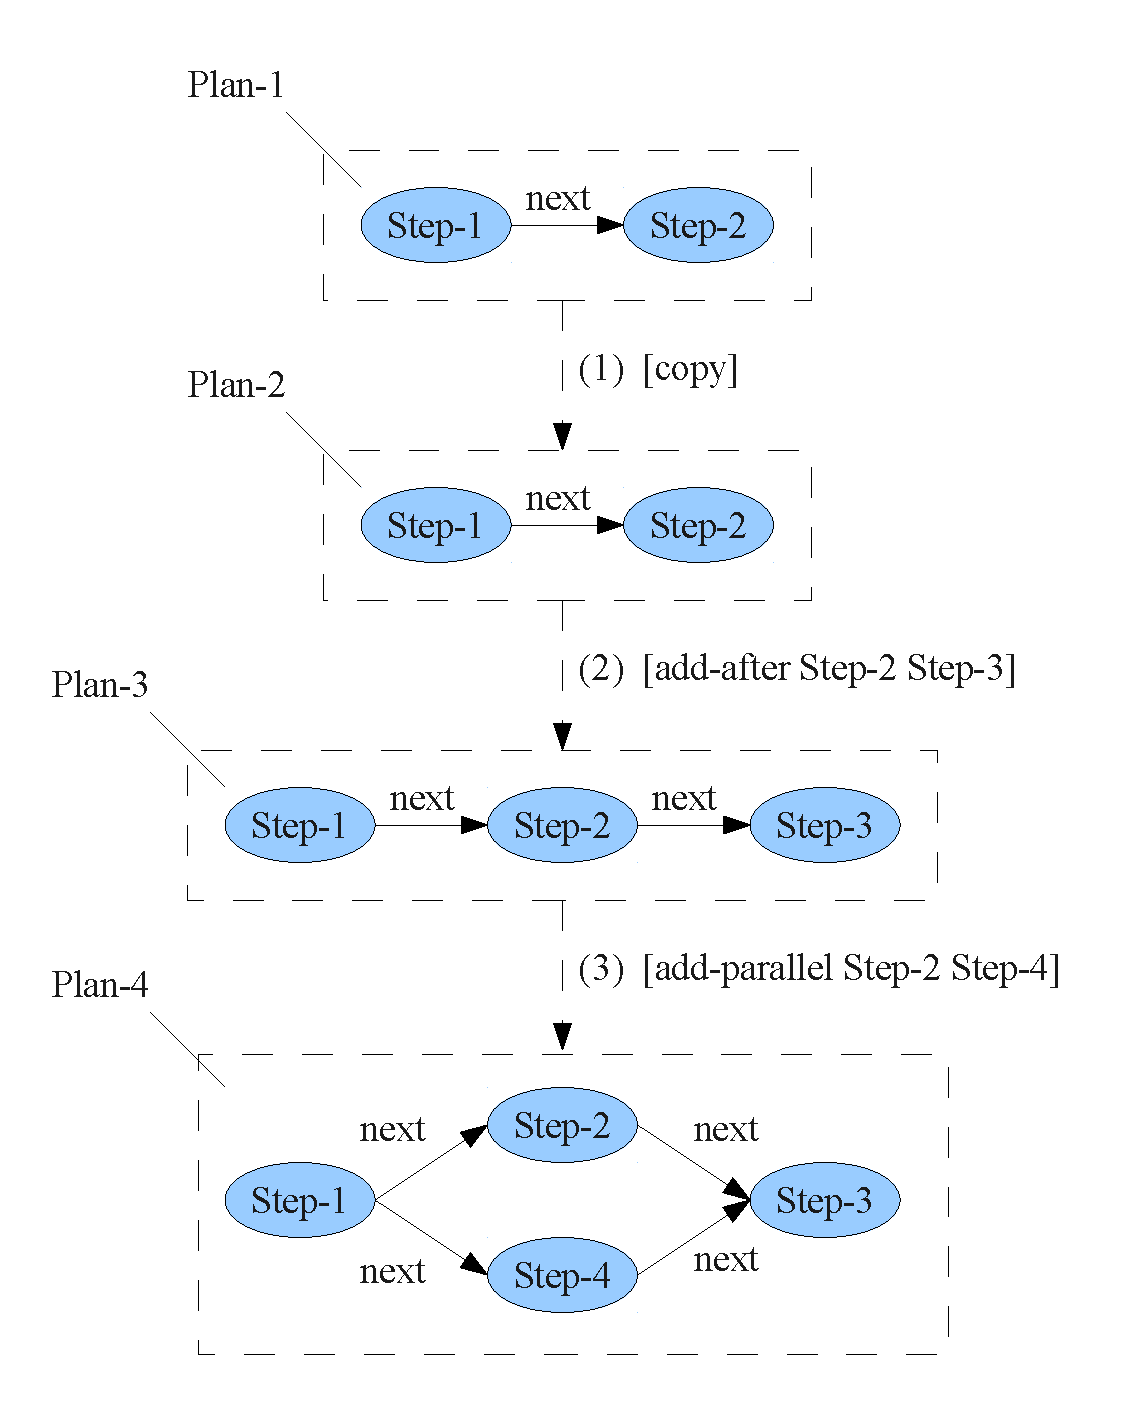
\includegraphics[height=8cm]{gfx/planning_machine_operations}
  \caption[A few planning machine operations.]{A few planning machine operations.}
  \label{fig:planning_machine_operations}
\end{figure}

A few operations for manupulating partially-ordered plans are shown in
Figure~\ref{fig:planning_machine_operations}.


\section{Planning Machine Reflective Knowledge}

\begin{figure}[bth]
  \center
  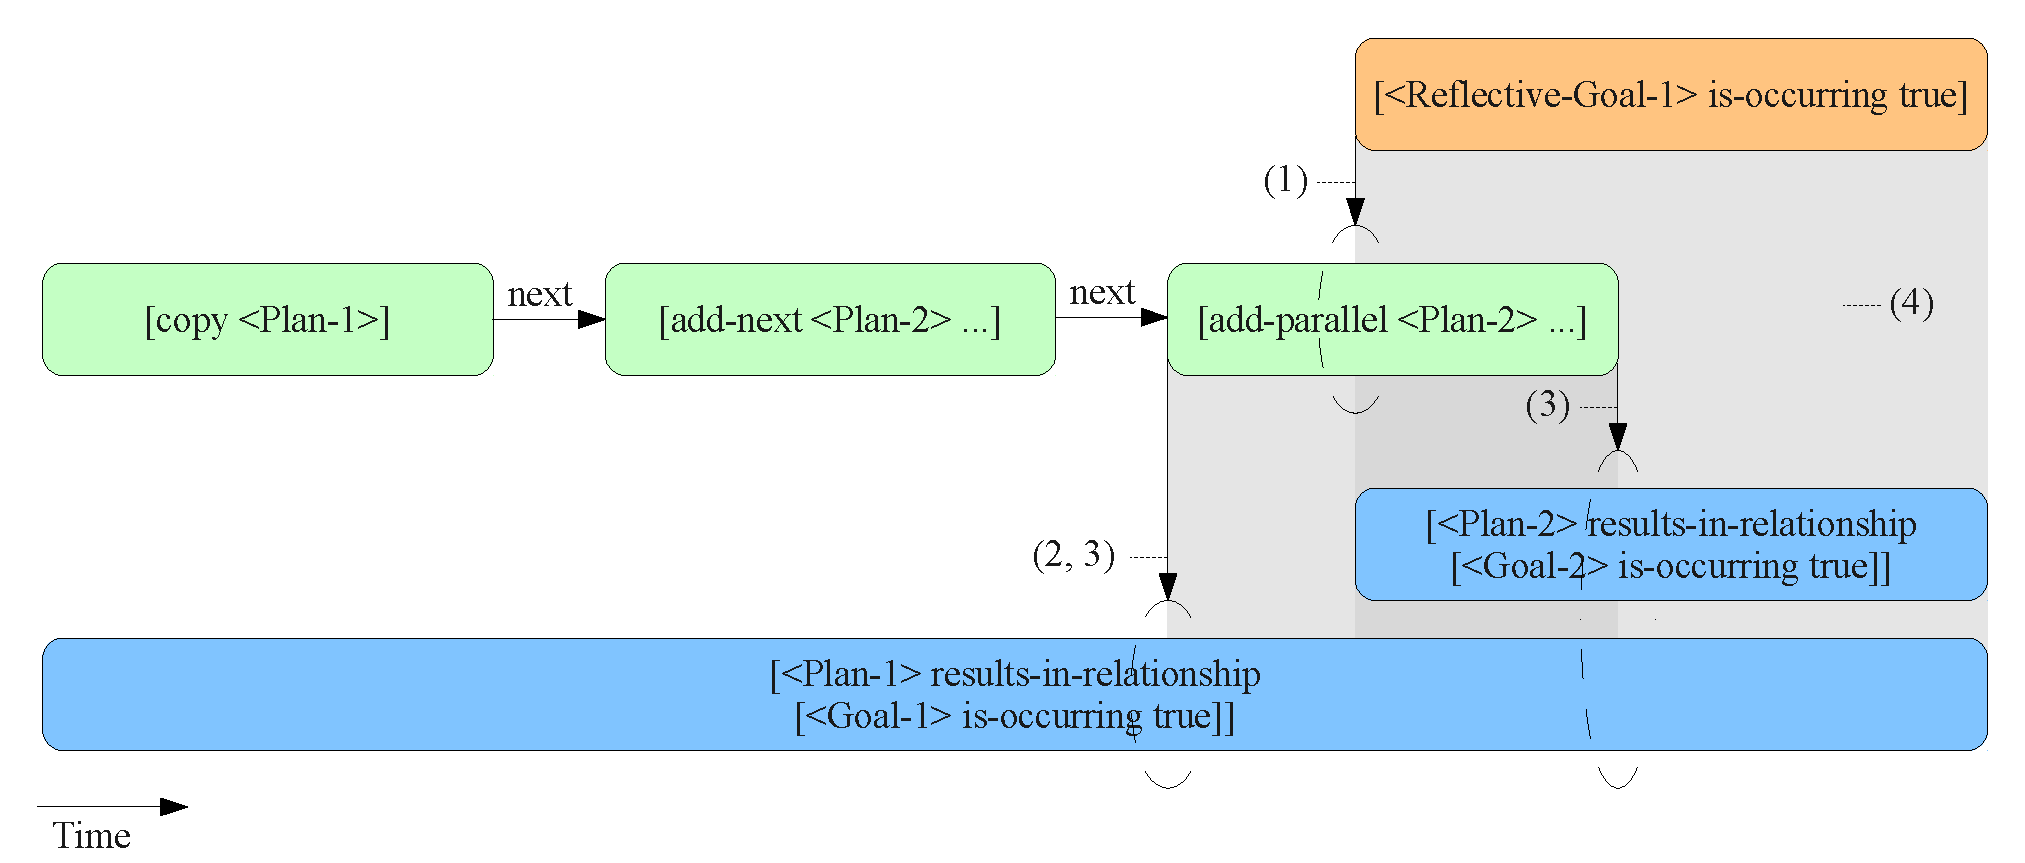
\includegraphics[width=11cm]{gfx/planning_machine_reflective_knowledge}
  \caption[Planning machine reflective knowledge.]{Planning machine reflective knowledge.}
  \label{fig:planning_machine_reflective_knowledge}
\end{figure}

See Figure~\ref{fig:planning_machine_reflective_knowledge}.

